\section{Only valid programs are alllowed to run}
\label{sec:valid}

\paragraph{Kinding validates types}

\freest{} requires kinding; GV does not. And the reason lies on
polymorphism, not on context-free types.
%
\lstinline|!Int| is undoubtedly a session type, and so is
\lstinline|!Int;?Bool|. On the other hand, \lstinline|Int->Bool| and
\lstinline|(Int,Bool)| are certainly funcional types. GV allows a
stratified grammar with separate syntactic categories for functional
types and for session types, even if mutually recursive.

Now let \lstinline|alpha| be a type variable. Is
\lstinline|!Int;alpha| a session type? What about \lstinline|alpha|
itself? The former is a session type only when \lstinline|alpha|
represents a session type; the latter is a functional type when
\lstinline|alpha| denotes a functional type, and a session type
otherwise. If \lstinline|alpha| does not denote a session type, then
\lstinline|!Int;alpha| is not a type, its simply a piece of useless
syntax.

\begin{wrapfigure}{R}{0.12\textwidth}
  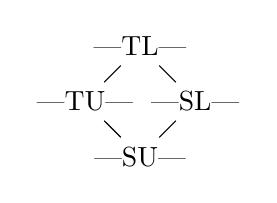
\begin{tikzpicture}[scale=.7]
    \node (TL) at (0,1) {\lstinline|TL|};
    \node (TU) at (-1,0) {\lstinline|TU|};
    \node (SL) at (1,0) {\lstinline|SL|};
    \node (SU) at (0,-1) {\lstinline|SU|};
    \draw (TL) -- (TU) -- (SU) -- (SL) -- (TL);
  \end{tikzpicture}
\end{wrapfigure}
%
Types, type variables included, are classified into \emph{kinds}. 
%
Kinds classify types. Kinds are pairs composed of a \emph{prekind} and
a \emph{multiplicity}. Prekinds distinguish functional types,
\lstinline|T|, from session types, \lstinline|S|.
%
Multiplicities control the number of times a value may be used in a
given context: exactly one---linear, \lstinline|L|---or zero or
more---unrestricted, \lstinline|U|. Both prekinds and multiplicities
come equipped with an ordering relation. Together they form the
lattice in the diagram on the right.
%
Types of kind \lstinline|TU| can be used at kind
\lstinline|TL|. Similarly, types of kind \lstinline|SU| can be used
at kind \lstinline|SL|. Any type can be seen at type \lstinline|TL|.

We are now in a better position to understand the type signature for
the functions in Section~\ref{sec:programming}.  Polymorphic variables
are solely introduced with the \lstinline|forall| construct. The
non-abbreviated type for function \lstinline|treeSum| is as follows.
%
\begin{lstlisting}
forall alpha:SL => Tree -> TreeC;alpha -> (Tree,alpha)
\end{lstlisting}
%
The absence of an explicit kinding is understood as \lstinline|SL|. In
this particular case, one can replace \lstinline|alpha| by any type
with a smaller or equal kind, including \lstinline|Skip : SU|, and
\lstinline|?Int;alpha : SL| in the examples in
Section~\ref{sec:programming}.

%%% Local Variables:
%%% mode: latex
%%% TeX-master: "main"
%%% End:
